\documentclass[11pt,letterpaper]{article}
\usepackage[T1]{fontenc}
\usepackage[scaled]{helvet}
\renewcommand{\familydefault}{\sfdefault}
\usepackage{amsmath,amssymb}
\usepackage[margin=0.8in,bottom=0.9in]{geometry}
\usepackage[most]{tcolorbox}
\usepackage{tikz}
\usetikzlibrary{calc}
\usepackage{enumitem}
\usepackage{array}
\usepackage{needspace}
\usepackage{fancyhdr}
\usepackage{pifont}

% ---- Palette "F. Bright & Playful" ----
\definecolor{fmtitle}{HTML}{3D2C8D}
\definecolor{fmkey}{HTML}{0096C7}
\definecolor{fmwatch}{HTML}{2BB673}
\definecolor{fmturn}{HTML}{F4A100}
\definecolor{fmmistake}{HTML}{EF476F}
\definecolor{fmnotice}{HTML}{9B5DE5}
\definecolor{fmgray}{HTML}{6B6B6B}

\pagestyle{fancy}
\fancyhf{}
\renewcommand{\headrulewidth}{0pt}
\fancyfoot[C]{\footnotesize\color{fmgray}\textcopyright\ 2026 FangMath. All rights reserved.}
\fancyfoot[R]{\footnotesize\color{fmgray}\thepage}
\setlength{\parindent}{0pt}
\setlength{\parskip}{3pt}

\newcommand{\badge}[1]{\colorbox{fmtitle}{\color{white}\bfseries\small\ #1\ }}
\newcommand{\leveltag}[2]{\colorbox{#1}{\color{white}\bfseries\scriptsize\ #2\ }}
\newcommand{\LE}{\leveltag{fmwatch}{EASY}}
\newcommand{\LM}{\leveltag{fmturn}{MEDIUM}}
\newcommand{\LH}{\leveltag{fmmistake}{HARD}}

\newcommand{\sectionbar}[2]{\needspace{6cm}\par\vspace{4mm}
  \begin{tcolorbox}[enhanced,colback=fmtitle,colframe=fmtitle,arc=2mm,
    left=4mm,top=1.5mm,bottom=1.5mm]
  \color{white}\bfseries\large #1\hfill{\normalsize\mdseries #2}
  \end{tcolorbox}}

\newtcolorbox{keyidea}{enhanced,breakable,colback=white,colframe=fmkey,boxrule=1pt,arc=2mm,
  title={Key Idea},coltitle=fmkey,fonttitle=\bfseries,
  attach boxed title to top left={xshift=4mm,yshift=-2mm},
  boxed title style={colback=white,colframe=fmkey,boxrule=0.9pt}}
\newtcolorbox{watchme}{enhanced,colback=white,colframe=fmwatch,boxrule=1pt,arc=2mm,
  title={Watch Me --- Worked Example},coltitle=fmwatch,fonttitle=\bfseries,
  attach boxed title to top left={xshift=4mm,yshift=-2mm},
  boxed title style={colback=white,colframe=fmwatch,boxrule=0.9pt}}
\newtcolorbox{mistakebox}{enhanced,breakable,colback=white,colframe=fmmistake,boxrule=1pt,arc=2mm,
  title={Common Mistake},coltitle=fmmistake,fonttitle=\bfseries,
  attach boxed title to top left={xshift=4mm,yshift=-2mm},
  boxed title style={colback=white,colframe=fmmistake,boxrule=0.9pt}}
\newtcolorbox{yourturn}{enhanced,breakable,colback=white,colframe=fmturn,boxrule=1pt,arc=2mm,
  title={Your Turn},coltitle=fmturn,fonttitle=\bfseries,
  attach boxed title to top left={xshift=4mm,yshift=-2mm},
  boxed title style={colback=white,colframe=fmturn,boxrule=0.9pt}}
\newtcolorbox{answerbox}[1]{enhanced,breakable,colback=white,colframe=fmwatch,boxrule=1pt,arc=2mm,
  title={#1},coltitle=fmwatch,fonttitle=\bfseries,
  attach boxed title to top left={xshift=4mm,yshift=-2mm},
  boxed title style={colback=white,colframe=fmwatch,boxrule=0.9pt}}

\newcommand{\work}[1]{\par\vspace{#1}}
\setlist[enumerate]{itemsep=2pt,topsep=3pt}

% ---------------- extra boxes ----------------
\newtcolorbox{notebox}{enhanced,breakable,colback=white,colframe=fmnotice,boxrule=1pt,arc=2mm,
  title={Notice},coltitle=fmnotice,fonttitle=\bfseries,
  attach boxed title to top left={xshift=4mm,yshift=-2mm},
  boxed title style={colback=white,colframe=fmnotice,boxrule=0.9pt}}
\newtcolorbox{exbox}{enhanced,colback=white,colframe=fmwatch,boxrule=0.8pt,arc=2mm,
  title={Example},coltitle=fmwatch,fonttitle=\bfseries\small,
  attach boxed title to top left={xshift=4mm,yshift=-2mm},
  boxed title style={colback=white,colframe=fmwatch,boxrule=0.8pt},fontupper=\small}
\newcommand{\topicbar}[1]{\needspace{4.5cm}\par\vspace{5mm}
  \begin{tcolorbox}[enhanced,colback=fmtitle,colframe=fmtitle,arc=2mm,left=4mm,top=1.5mm,bottom=1.5mm]
  \color{white}\bfseries\large #1
  \end{tcolorbox}}
\usepackage{multicol}

% ---------------- practice layout ----------------
\newcommand{\workline}{\par\vspace{7mm}{\color{gray!55}\rule{\linewidth}{0.4pt}}}
\newcommand{\worklines}[1]{\foreach \i in {1,...,#1}{\workline}}
\newcommand{\prob}[3]{\needspace{#3}\par\vspace{3mm}{\color{fmturn}\bfseries #1.}\ #2\par}
\newcommand{\ansline}{\par\vspace{4mm}\hfill\textbf{Answer:}\ \rule{5cm}{0.4pt}\par}
\newcommand{\keyitem}[3]{\needspace{3.2cm}\par\vspace{2mm}
  \begin{tcolorbox}[enhanced,colback=white,colframe=fmwatch!60,boxrule=0.6pt,arc=1.5mm,left=3mm,top=1.5mm,bottom=1.5mm]
  {\color{fmwatch}\bfseries #1.}\quad\small #2\par\vspace{1mm}
  \normalsize\textbf{Answer: #3}
  \end{tcolorbox}}


\usetikzlibrary{arrows.meta}
\providecommand{\iskey}{0}
% fill-in blank: line for students, pink answer in the key
\newcommand{\fb}[2][2.6cm]{\ifnum\iskey=1 \underline{\makebox[#1][c]{\color{fmmistake}\bfseries #2}}\else\underline{\makebox[#1]{}}\fi}
% answer line for practice problems
\newcommand{\pans}[2][3.2cm]{\ifnum\iskey=1 \underline{\makebox[#1][c]{\color{fmmistake}\bfseries #2}}\else\rule{#1}{0.4pt}\fi}
\newcommand{\vid}[1]{{\color{fmgray}\small\textit{\ding{43} Video: #1}}}
\newcommand{\pt}[2]{\fill (#1) circle (2.2pt) node[above=1pt,font=\small]{$#2$};}

\usetikzlibrary{decorations.pathreplacing}
\newcommand{\gridb}[4]{\draw[gray!30,step=1] (#1,#2) grid (#3,#4);\draw[gray!70,-{Stealth}] (#1,0)--(#3+0.4,0);\draw[gray!70,-{Stealth}] (0,#2)--(0,#4+0.4);}
\newcommand{\sdp}[3]{\begin{minipage}[t][2.4cm]{0.48\linewidth}{\color{fmturn}\bfseries #1.}\ #2\par\vfill\hfill \pans[3.6cm]{#3}\end{minipage}}
\newcommand{\sdpw}[3]{\begin{minipage}[t][2.4cm]{0.48\linewidth}{\color{fmturn}\bfseries #1.}\ #2\par\vfill\hfill \pans[5.2cm]{#3}\end{minipage}}
\newcommand{\algp}[3]{\begin{minipage}[t][4.2cm]{0.48\linewidth}{\color{fmturn}\bfseries #1.}\ #2\par\vfill\hfill \pans[4.4cm]{#3}\end{minipage}}
\newcommand{\pair}[2]{\needspace{3.4cm}\noindent #1\hfill #2\par\vspace{2mm}}
\newcommand{\head}[2]{\ifnum\iskey=1 \colorbox{fmwatch}{\color{white}\bfseries\small\ ANSWER KEY\ }\else\badge{#1}\fi\hfill{\small\color{fmgray}Geometry \textperiodcentered\ Lesson #2}\par\vspace{4mm}}
\newcommand{\nameline}{Name: \rule{6cm}{0.4pt}\hspace{1cm}Date: \rule{3.5cm}{0.4pt}\par\vspace{2mm}}
\renewcommand{\vid}[1]{\needspace{4.2cm}{\color{fmgray}\small\textit{\ding{43} Video: #1}}}
\begin{document}
\head{PRACTICE}{1.5}
{\color{fmtitle}\LARGE\bfseries Angles --- Practice\ifnum\iskey=1 \ --- Answer Key\fi}\par\vspace{1mm}
{\color{fmgray}A worked example comes before each type. Show your thinking.}\par\vspace{3mm}
\nameline

\needspace{6cm}\topicbar{Type 1 \quad Classify the Angle}
\begin{watchme}Classify an angle of $132^\circ$.\par
It is more than $90^\circ$ but less than $180^\circ$. \quad \textbf{Answer: obtuse}\end{watchme}
\pair{\sdp{1}{$47^\circ$}{acute}}{\sdp{2}{$90^\circ$}{right}}
\pair{\sdp{3}{$179^\circ$}{obtuse}}{\sdp{4}{$180^\circ$}{straight}}

\needspace{6.5cm}\topicbar{Type 2 \quad Angle Addition Postulate}
\begin{watchme}$D$ is inside $\angle ABC$. $m\angle ABD = 28^\circ$ and $m\angle DBC = 47^\circ$. Find $m\angle ABC$.\par
Part $+$ part $=$ whole: $28 + 47 = 75$. \quad \textbf{Answer: $\boldsymbol{75^\circ}$}\end{watchme}
\pair{\sdp{5}{$m\angle ABD = 40^\circ$, $m\angle DBC = 65^\circ$. Find $m\angle ABC$.}{$105^\circ$}}{\sdp{6}{$m\angle ABC = 120^\circ$, $m\angle ABD = 45^\circ$. Find $m\angle DBC$.}{$75^\circ$}}
\needspace{4.6cm}\noindent\algp{7}{$m\angle ABD = x + 10$, $m\angle DBC = 2x + 5$, $m\angle ABC = 90^\circ$. Find $x$ and $m\angle DBC$.}{$x = 25,\ 55^\circ$}\hfill\algp{8}{\LH\ $\overrightarrow{BD}$ bisects $\angle ABC$. $m\angle ABD = 3x + 4$, $m\angle DBC = 5x - 12$. Find $m\angle ABC$.}{$x = 8,\ 56^\circ$}\par

\needspace{6.5cm}\topicbar{Type 3 \quad Complements \& Supplements}
\begin{watchme}Find the complement and the supplement of $38^\circ$.\par
Complement: $90 - 38 = 52^\circ$. \ Supplement: $180 - 38 = 142^\circ$. \quad \textbf{Answer: $\boldsymbol{52^\circ}$, $\boldsymbol{142^\circ}$}\end{watchme}
\pair{\sdp{9}{Find the complement of $71^\circ$.}{$19^\circ$}}{\sdp{10}{Find the supplement of $98^\circ$.}{$82^\circ$}}
\needspace{4.6cm}\noindent\algp{11}{Two angles are complementary. One is twice the other. Find both.}{$30^\circ,\ 60^\circ$}\hfill\algp{12}{Two angles are supplementary: $x$ and $3x - 20$. Find both.}{$50^\circ,\ 130^\circ$}\par

\needspace{7cm}\topicbar{Type 4 \quad Vertical Angles \& Linear Pairs}
\begin{watchme}\begin{minipage}[c]{0.3\linewidth}\centering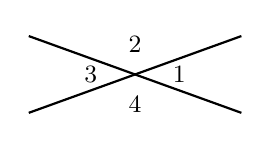
\begin{tikzpicture}[scale=0.75]
\draw[thick] (-1.8,-0.65)--(1.8,0.65);\draw[thick] (-1.8,0.65)--(1.8,-0.65);
\node[font=\small] at (0.75,0){$1$};\node[font=\small] at (0,0.5){$2$};\node[font=\small] at (-0.75,0){$3$};\node[font=\small] at (0,-0.5){$4$};\end{tikzpicture}\end{minipage}\hfill
\begin{minipage}[c]{0.66\linewidth}$m\angle 1 = 65^\circ$. Find $m\angle 3$ and $m\angle 2$.\par
Vertical angles are equal: $m\angle 3 = 65^\circ$. Linear pair: $m\angle 2 = 180 - 65 = 115^\circ$.\par
\textbf{Answer: $\boldsymbol{65^\circ}$, $\boldsymbol{115^\circ}$}\end{minipage}\end{watchme}
{\small Use the picture in the example for problems 13 and 14.}\par
\pair{\sdp{13}{$m\angle 2 = 128^\circ$. Find $m\angle 4$.}{$128^\circ$}}{\sdp{14}{$m\angle 1 = 73^\circ$. Find $m\angle 2$.}{$107^\circ$}}
\needspace{4.6cm}\noindent\algp{15}{Vertical angles measure $5x - 10$ and $3x + 30$. Find $x$ and the angle.}{$x = 20,\ 90^\circ$}\hfill\algp{16}{A linear pair measures $2x + 15$ and $3x - 5$. Find both angles.}{$83^\circ,\ 97^\circ$}\par
\end{document}
